\documentclass{article}
\usepackage[hyphens]{url}
\usepackage{mathtools}
\usepackage{amsmath}
\usepackage{listings}
\usepackage{graphicx}
\usepackage[margin=1in]{geometry}
\usepackage{float}
\floatstyle{boxed}
\restylefloat{figure}
\lstset{breaklines=true}
\begin{document}


\title{CS595 Intro to Web Science, Assignment \#4}
\author{Valentina Neblitt-Jones}
\date{October 10, 2013}
\maketitle

\section*{Question 1}

From your list of 1000 links, choose 100 and extract all of the links from those 100 pages to other pages. We're looking for user navigable links, that is in the form of:  \\

\begin{verbatim}
<a href = "foo">bar</a>
\end{verbatim}

We're not looking for embedded images, scripts, <link> elements, etc. You'll probably want to use BeautifulSoup for this. \\

For each URI, create a text file of all the outbound links from that page to other URIs (use any syntax that is easy for you). For example: \\

site:
\url{http://www.cs.odu.edu/~mln/}

links:
\url{http://www.cs.odu.edu/}
\url{http://www.odu.edu}
\url{http://www.cs.odu.edu/~mln/research/}
\url{http://www.cs.odu.edu/~mln/pubs/}
\url{http://ws-dl.blogspot.com/}
\url{http://ws-dl.blogspot.com/2-13/09/2013-09-09-ms-thesis-http-mailbox.html}
etc. \\

Upload these 100 files to github (they don't have to be in your report).

\subsection*{Answer to Question 1}

I selected 100 links from the finding aid in Assignment \#2 from the following agencies:

\begin{itemize}
\item TMZ.com
\item Sesame Workshop
\item VT News
\item Washington City Paper
\item Library of Congress 
\end{itemize}

Figure \ref{inputfile} showed a sample of the input file. It has the md5 and the URI for each link.

\begin{figure}[H]
\centering
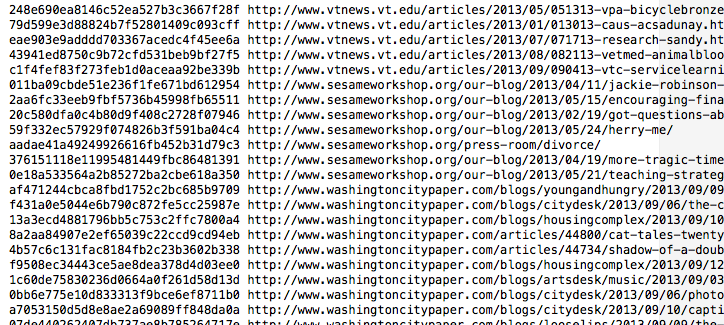
\includegraphics[scale=0.50]{q1/inputfile}
\caption{Sample of Input File}
\label{inputfile}
\end{figure}

My Python code (Figure \ref{extractlinks}) split each line of the input file into two variables called rawfile and uri. As suggested, I used BeautifulSoup to find all the links in the file. Outputting the links was a little tricky since using the simple example below at \url{www.pythonforbeginners.com/python-on-the-web/beautifulsoup-4-python}, represented relative links as they are in the file and I needed full links.

\begin{verbatim}

from bs4 import BeautifulSoup
import urllib2
 
redditFile = urllib2.urlopen("http://www.reddit.com")
redditHtml = redditFile.read()
redditFile.close()
 
soup = BeautifulSoup(redditHtml)
redditAll = soup.find_all("a")
for links in soup.find_all('a'):
    print (links.get('href'))

\end{verbatim}

So I needed to take care of a few cases and urlparse was needed to break the uri into its key components as explained in Python documentation \url{http://docs.python.org/2/library/urlparse.html} - scheme, netloc and path. It checks if the link is relative. If it is relative then it should add the scheme from the parent page and the netloc from the parent page. There was also the matter of extra slashes. Some links already had a slash and others did not. I need it to add the slash if it was not already there and there was a path. I also needed it to throw out any javascript that was picked up by BeautifulSoup. I formatted the output files as suggested in the assignment description (Figure \ref{sampleoutputfile}).

\begin{figure}[H]
\centering
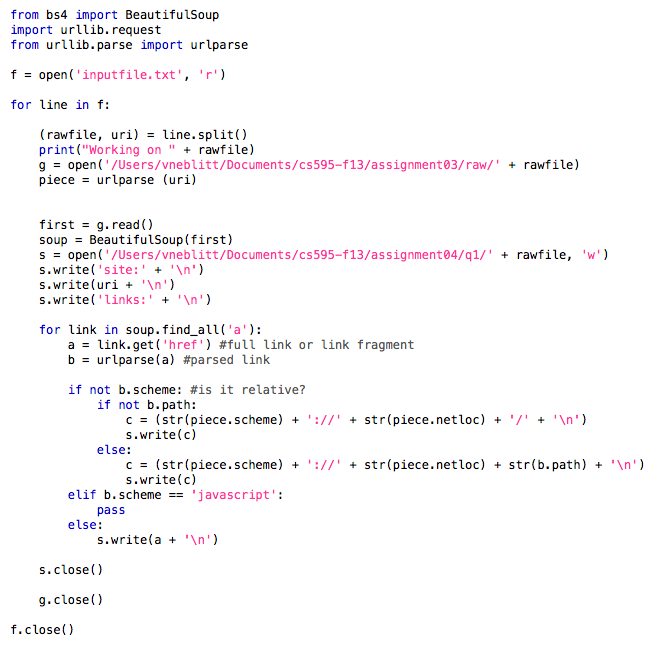
\includegraphics[scale=0.60]{q1/extractlinkscode}
\caption{ExtractLinks.py}
\label{extractlinks}
\end{figure}

\begin{figure}[H]
\centering
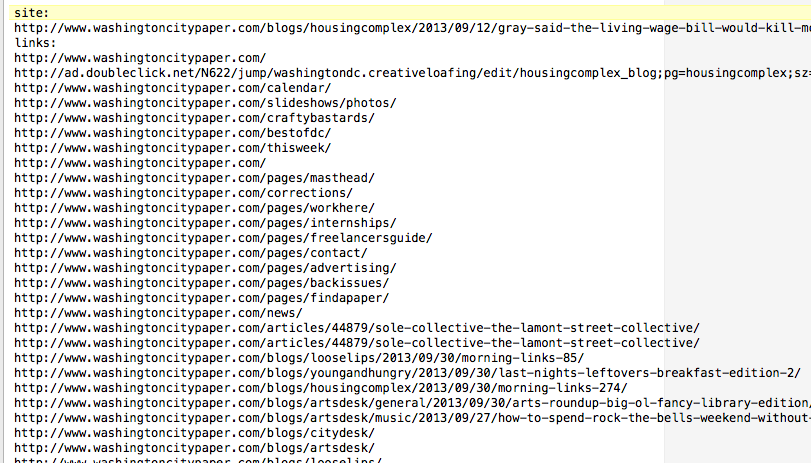
\includegraphics[scale=0.50]{q1/sampleoutputfile}
\caption{Sample of an Output File}
\label{sampleoutputfile}
\end{figure}

%\begin{figure}[H]
%\centering
%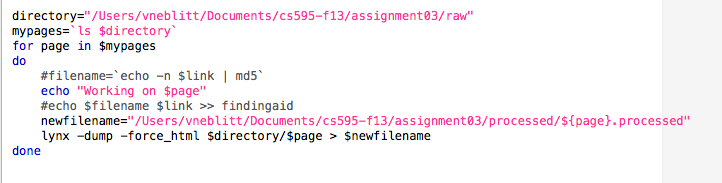
\includegraphics[scale=0.50]{q1/rmMarkupURI}
%\caption{Shell Script to Remove Markup}
%\label{rmMarkup}
%\end{figure}

\newpage

\section*{Question 2}

Using these 100 files, create a single GraphViz ``dot'' file of the resulting graph. Learn about dot at: \\

Examples:
\begin{itemize}
\item \url{http://www.graphviz.org/content/unix}
\item \url{http://www.graphviz.org/Gallery/directed/unix.gv.txt}
\end{itemize}

Manual:
\begin{itemize}
\item \url{http://www.graphviz.org/Documentation/dotguide.pdf}
\end{itemize}

Reference:
\begin{itemize}
\item \url{http://www.graphviz.org/content/dot-language}
\item \url{http://www.graphviz.org/Documentation.php}
\end{itemize}

Note: You'll have to put explicit labels on the graph, see: \url{https://gephi.org/users/supported-graph-formats/graphviz-dot-format/} \\

Note: Actually, I'll allow any of the formats listed here: \url{https://gephi.org/users/supported-graph-formats/}, but ``dot'' is probably the simplest.

%\begin{table}[!h]
%\centering
%\caption{10 Hits for the term ``shadow'', ranked by TFIDF}
%\begin{tabular}{c c c c}
%\hline
%TFIDF & TF & IDF & URI \\
%\hline
%\hline
%0.150 & 0.014 & 10.680 & http://foo.com \\
%0.085 & 0.008 & 10.680 & http://bar.com \\
%\hline
%\end{tabular}
%\end{table}

\subsection*{Answer to Question 2}

Since I needed to iterate through a file directory I needed to use listdir from os. I found guidance for using this on a tutorial page \url{http://www.tutorialspoint.com/python/os_listdir.htm}.

\begin{verbatim}
import os, sys

# Open a file
path = "/var/www/html/"
dirs = os.listdir( path )

# This would print all the files and directories
for file in dirs:
   print file
\end{verbatim}

I tested this in the IDLE Python shell and found out that the .DS\_Store file would be included. Rather than find out what my code would do with that file I chose to remove it. So in my code (Figure \ref{createdotfile}), I started with a modification of the code above to create the list that the rest of my code would iterate through. Basically I needed to skip the first line of the file which just had the word ``site:''. Then I wanted to make the second line in the file a variable called site. Next I needed to skip the third line in the file which just had the word ``link''. Finally, I needed the fourth line until the end of the file to be stored as links. The code output the site and relates it to the link and adds the label. As it ran through the files, I needed everything to end up in a single document ``mydotfile.dot'' and named the digraph ``spaghetti''. Figure \ref{dotfileexample} shows a sample of the dot file produced.

\begin{figure}[H]
\centering
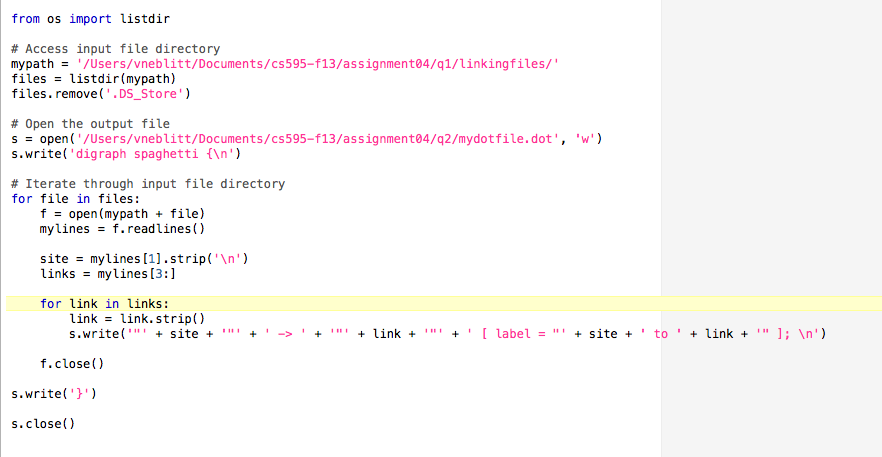
\includegraphics[scale=0.50]{q2/createdotfilecode}
\caption{CreateDotFile.py}
\label{createdotfile}
\end{figure}

\begin{figure}[H]
\centering
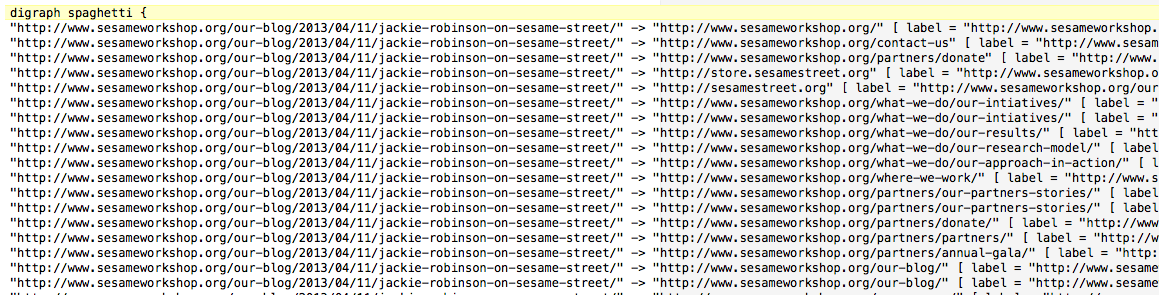
\includegraphics[scale=0.40]{q2/sampledotfileoutput}
\caption{Sample of the Dot File Output}
\label{dotfileexample}
\end{figure}

\clearpage

\section*{Question 3}
Download and install Gephi: \\
\url{}

Load the dot file created in \#2 and use Gephi to:
\begin{itemize}
\item visualize the graph (you'll have to turn on labels)
\item calculate HITS and PageRank
\item avg degree
\item network diameter
\item connected components
\end{itemize}

Put the resulting graphs in your report. \\

You might need to choose the 100 sites with an eye toward creating a graph with at least one component that is nicely connected. You can probably do this be selecting some portion of your links (e.g., 25, 50) from the same site.

\subsection*{Answer to Question 3}

I downloaded Gephi and imported my dot file. The first result was called in the email list a hairball, but I thought dirty pillow was another good description (Figure \ref{dirtypillow}). I attempted several layouts, but there results did not illustrate much. I used Force Atlas and the graph started spreading out too far to still be represented in a report. The nodes for VT News and Washington City Paper managed to be totally separated from other groupings. However there was some connection between Library of Congress, TMZ, and Sesame Workshop. In Figure \ref{forceatlas}, the grouping in the top right represents VT News. The grouping in the top left represents Washington City Paper. The center groupings are Library of Congress (left) and Sesame Workshop (right). The bottom grouping is TMZ.

I ran the requested reports as well. The report names matched the titles in the assignment description with the exception of network diameter. The tool called it Network Diameter (Figure \ref{gephiinterface}), but the reports were labeled Graph Distance. There was not much to see in the reports, but it seems that we did not have enough data to populate those charts.

\subsubsection*{Visualizations}

\begin{figure}[H]
\centering
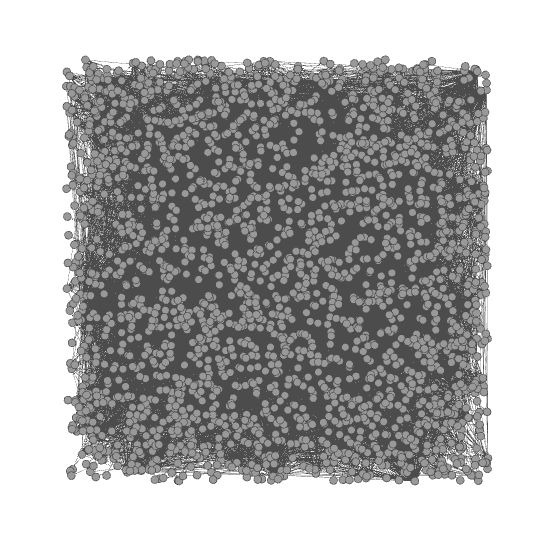
\includegraphics[scale=0.70]{q3/dirtypillow}
\caption{Dirty Pillow}
\label{dirtypillow}
\end{figure}

\begin{figure}[H]
\centering
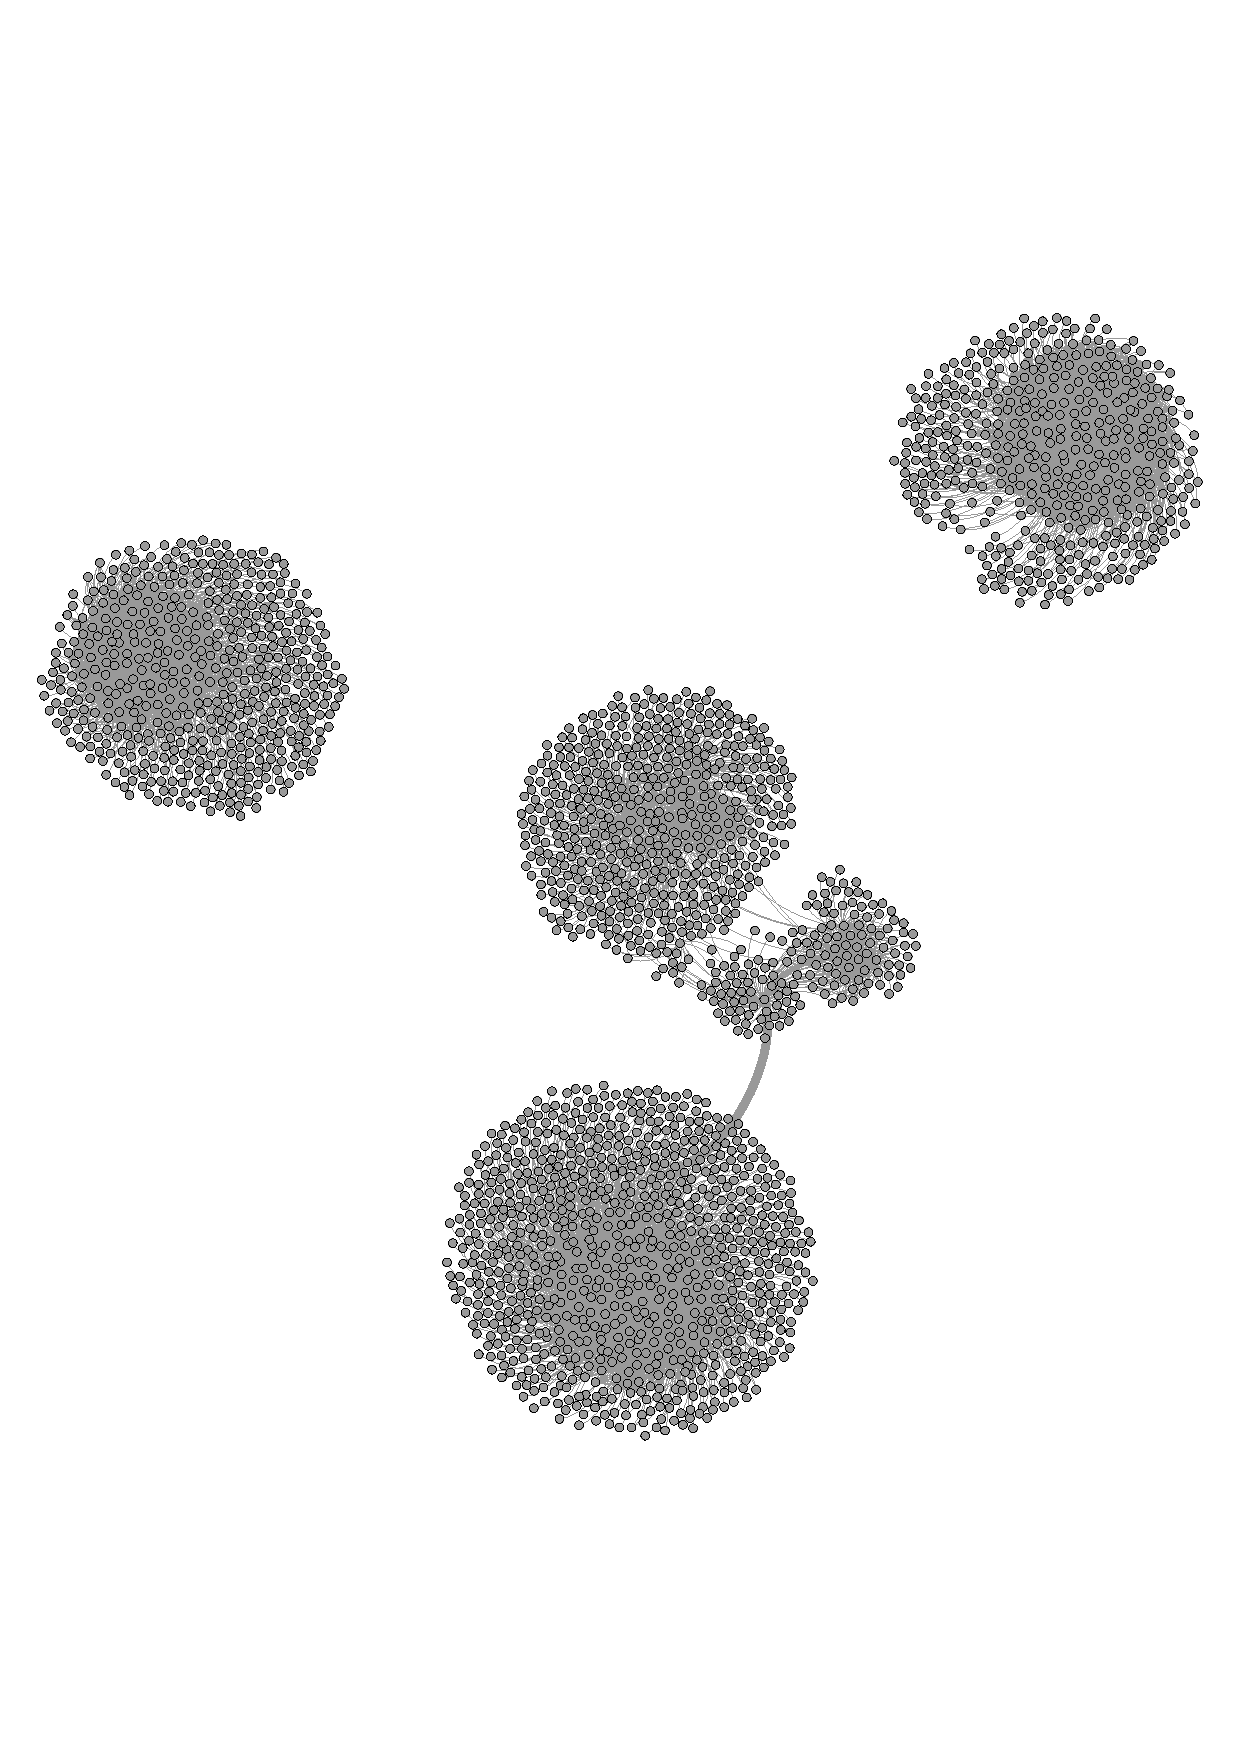
\includegraphics[scale=0.60]{q3/visualization02}
\caption{Visualization with Force Atlas 2}
\label{forceatlas}
\end{figure}

\begin{figure}[H]
\centering
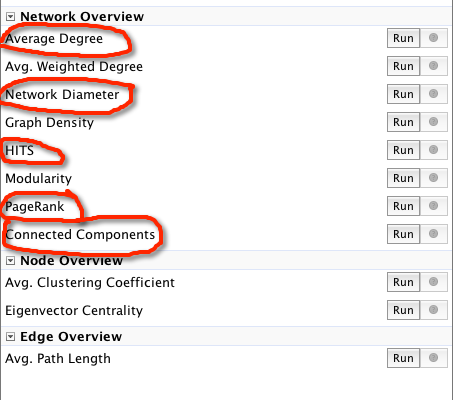
\includegraphics[scale=0.70]{q3/gephireports}
\caption{Gephi Reports Interface}
\label{gephiinterface}
\end{figure}

\subsubsection*{HITS Metric Report}

\begin{figure}[H]
\centering
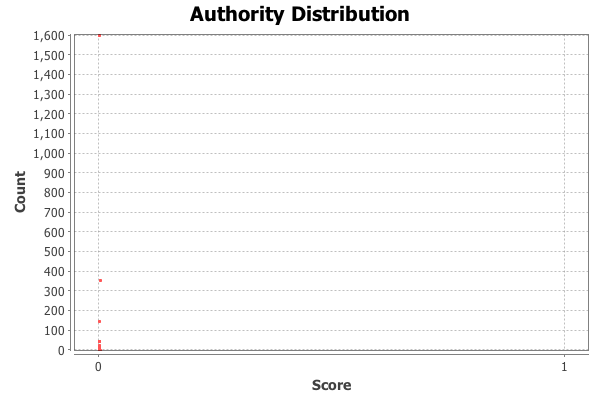
\includegraphics[scale=0.70]{q3/HitsMetricReport/authorities}
\caption{Authority Distribution}
\label{authoritydistribution}
\end{figure}

\begin{figure}[H]
\centering
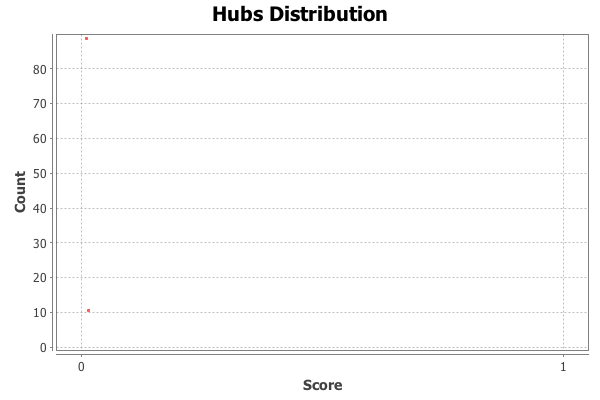
\includegraphics[scale=0.70]{q3/HitsMetricReport/hubs}
\caption{Hubs Distribution}
\label{hubsdistribution}
\end{figure}

\subsubsection*{PageRank Report}

\begin{figure}[H]
\centering
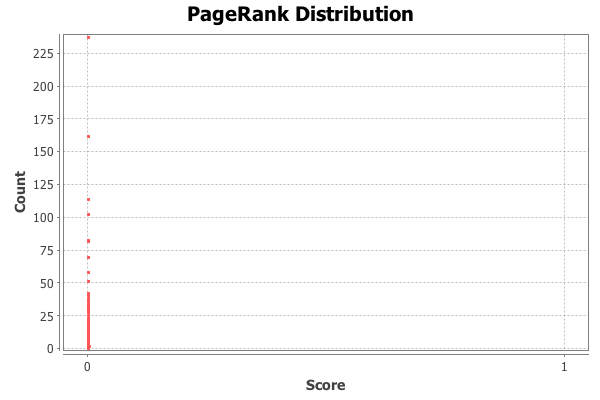
\includegraphics[scale=0.70]{q3/PageRankReport/pageranks}
\caption{PageRank Distribution}
\label{pageranks}
\end{figure}

\subsubsection*{Average Degree Reports}

\begin{figure}[H]
\centering
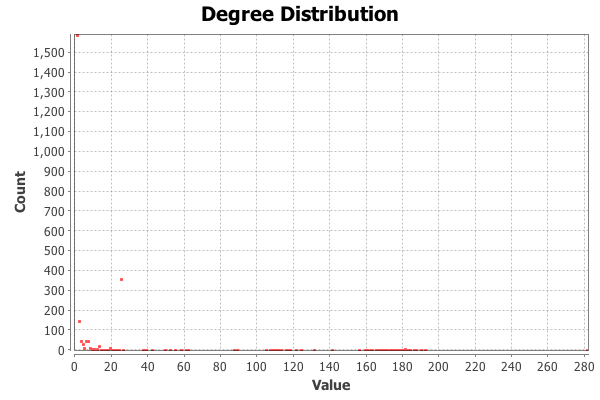
\includegraphics[scale=0.70]{q3/AverageDegreeReport/degree-distribution}
\caption{Degree Distribution}
\label{degreedistribution}
\end{figure}

\begin{figure}[H]
\centering
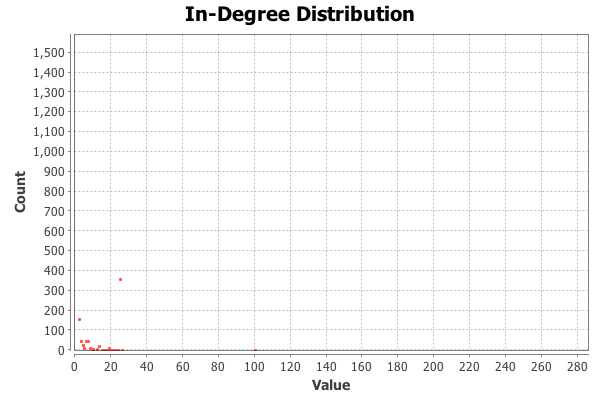
\includegraphics[scale=0.70]{q3/AverageDegreeReport/indegree-distribution}
\caption{In-Degree Distribution}
\label{degreedistribution}
\end{figure}

\begin{figure}[H]
\centering
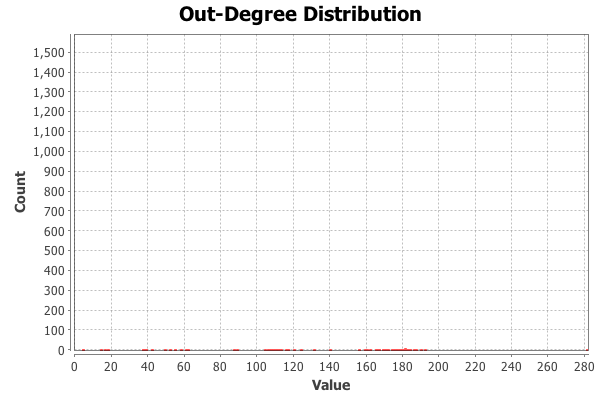
\includegraphics[scale=0.70]{q3/AverageDegreeReport/outdegree-distribution}
\caption{Out-Degree Distribution}
\label{degreedistribution}
\end{figure}

\subsubsection*{Graph Distance Report}

\begin{figure}[H]
\centering
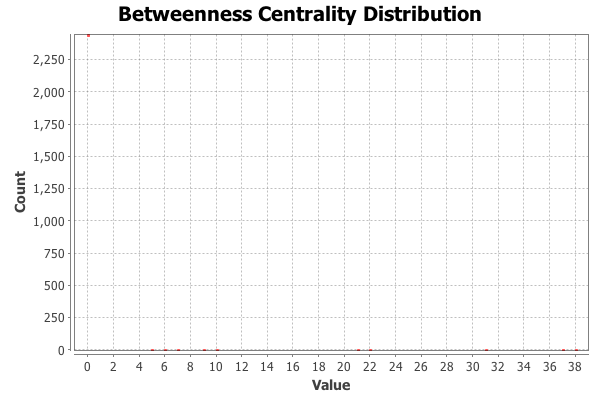
\includegraphics[scale=0.70]{q3/GraphDistanceReport/BetweennessCentralityDistribution}
\caption{Betweenness Centrality Distribution}
\label{businesscentrality}
\end{figure}

\begin{figure}[H]
\centering
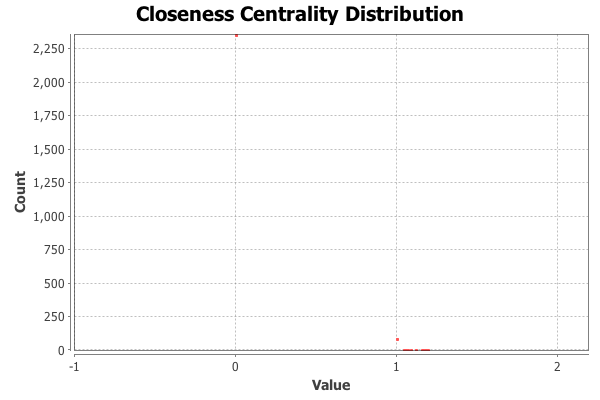
\includegraphics[scale=0.70]{q3/GraphDistanceReport/ClosenessCentralityDistribution}
\caption{Closeness Centrality Distribution}
\label{closeness centrality}
\end{figure}

\begin{figure}[H]
\centering
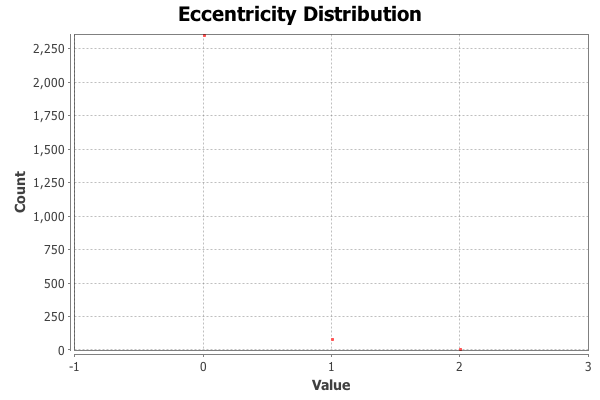
\includegraphics[scale=0.70]{q3/GraphDistanceReport/EccentricityDistribution}
\caption{Eccentricity Distribution}
\label{eccentricitydistribution}
\end{figure}

\subsubsection*{Connected Components Report}

\begin{figure}[H]
\centering
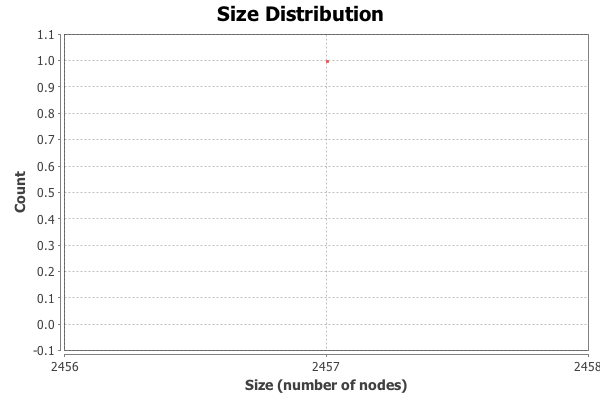
\includegraphics[scale=0.70]{q3/ConnectedComponentsReport/cc-size-distribution}
\caption{Size Distribution}
\label{sizedistribution}
\end{figure}

\end{document}